\lab{Algorithms}{Metropolis Algorithm}{Metropolis Algorithm}
\objective{Understand the basic principles of the Metropolis algorithm.}

Thus far when computing posterior distributions, we have dealt with scenarios in which the distributions take on a nice form, i.e. where the posterior distribution is of the same form as the prior. These are called \emph{conjugate prior} distributions. There are, however, times when computing the posterior distribution is not so simple. Often this arises due to our inability to efficiently compute the integral in the denominator of our typical use of Bayes Rule:
\begin{equation*}
\mathbb{P}(\theta | \mathbf{y}) = \frac{\mathbb{P}(\mathbf{y} | \theta) \mathbb{P}(\theta)}{\int \mathbb{P}(\mathbf{y} | \theta)\mathbb{P}(\theta) d\theta}
\end{equation*}
If we ignore the denominator, we can write 
\begin{equation*}
\mathbb{P}(\theta | \mathbf{y}) \propto \mathbb{P}(\mathbf{y} | \theta) \mathbb{P}(\theta)
\end{equation*}
which is often easier to compute.

The Metropolis algorithm provides us a method by which we can sample from the posterior distribution, provided that we can easily compute the right hand side of the above equation, which we will denote $f(\theta)$. This is done by constructing a Markov chain which is irreducible, non-null recurrent and aperiodic, which has $\mathbb{P}(\theta | \mathbf{y})$ as its unique invariant distribution.

We begin by choosing a simple Markov chain over the state space that has symmetric transition matrix $Q$, such that $Q(x | x) = 0$ for all $x$ in the state space. Obviously, for non-discrete state spaces, $Q$ is not really a matrix, but it must still define transition probabilities such that $Q(x | y) = Q(y | x)$. We then define an acceptance matrix $A$, where $A(x | y) = \min{1,\frac{f(x)}{f(y)}}$. Again, $A$ is not a matrix if the state space is not discrete, but it will be defined for all pairs $x,y$ in the state space.

We combine these to produce a Markov chain with transition probabilities
\begin{equation*}
H(x | y) = \begin{cases} Q(x | y)A(x | y) & \mbox{ if } x \neq y, \\ 1 - \sum_{y \neq x} Q(x | y)A(x | y) & \mbox{ if } x = y \end{cases}
\end{equation*}

Essentially, given our current state, we propose a new state according to $Q$. We then accept or reject it according to $A$, and continue the process. So long as $Q$ defines an irreducible, non-null recurrent, and aperiodic Markov chain, then $H$ will define a Markov chain whose unique invariant distribution will be $\mathbb{P}(\theta | \mathbf{y})$. Furthermore, given any initial state, the chain will converge to this invariant distribution.

What this means is that we can sample from the desired distribution after a ``burn-in'' period (to remove the effects of our initial state choice). We will use the Metropolis algorithm to obtain samples from a multivariate normal distribution to demonstrate this process.

Suppose we can easily sample from the multivariate normal distribution with mean $\mu$ and covariance matrix $I$, the identity. In Python, this is as follows:
\begin{lstlisting}
: import numpy as np
: mu = np.array([3., -5.])
: sigma = np.eye(2)
: sample = np.random.multivariate_normal(mu,sigma)
\end{lstlisting}

Suppose also that we desire to obtain samples from a multivariate normal distribution with arbitrary covariance matrix $\Sigma$, and that this is difficult (obviously we can do this directly in Python, but this is merely a tutorial to see how the Metropolis algorithm works). Suppose further that we are able to easily compute the ratio of the density of this distribution at two points $\mathbf{x}$ and $\mathbf{y}$ of length $K$, i.e.
\begin{align*}
\frac{N(\mathbf{x} \; ; \; \mu, \Sigma)}{N(\mathbf{y} \; ; \; \mu, \Sigma)} & = \frac{\frac{1}{(2\pi)^{K/2}|\Sigma|^{1/2}} e^{-\frac{1}{2}(\mathbf{x} - \mu)^{T} \Sigma^{-1} (\mathbf{x} - \mu)}}{\frac{1}{(2\pi)^{K/2}|\Sigma|^{1/2}} e^{-\frac{1}{2}(\mathbf{y} - \mu)^{T} \Sigma^{-1} (\mathbf{x} - \mu)}} \\
& = \frac{e^{-\frac{1}{2}(\mathbf{x} - \mu)^{T} \Sigma^{-1} (\mathbf{x} - \mu)}}{e^{-\frac{1}{2}(\mathbf{y} - \mu)^{T} \Sigma^{-1} (\mathbf{x} - \mu)}} \\
& = e^{-\frac{1}{2}\left((\mathbf{x} - \mu)^{T} \Sigma^{-1} (\mathbf{x} - \mu) - (\mathbf{y} - \mu)^{T} \Sigma^{-1} (\mathbf{y} - \mu)\right)}
\end{align*}

\begin{problem} \label{problem1}
Write an acceptance function that computes 
\begin{equation*}
p = \min \{1, e^{-\frac{1}{2}\left((\mathbf{x} - \mu)^{T} \Sigma^{-1} (\mathbf{x} - \mu) - (\mathbf{y} - \mu)^{T} \Sigma^{-1} (\mathbf{y} - \mu)\right)}\}
\end{equation*}
given $\mathbf{x}, \mathbf{y}, \mu,$ and $\Sigma$, and then draws from a Bernoulli distribution with parameter $p$. It should return a $1$ if it accepts the new state, and a $0$ if it rejects it.
\end{problem}

Specifically, we will try to sample from the distribution centered at the origin, with covariance matrix
\begin{equation*}
\Sigma = \left[ \begin{array}{cc} 12 & 4 \\ 4 & 16 \end{array} \right]
\end{equation*}

\begin{lstlisting}
: mu = np.zeros(2)
: sigma = np.array([[12., 10.], [10., 16.]])
\end{lstlisting}

We will let $Q(\mathbf{x} | \mathbf{y}) = N(\mathbf{x} \; ; \; \mathbf{y}, I)$ be our proposal distribution, given that we are currently in state $\mathbf{y}$, i.e. we propose a new state by drawing from the multivariate normal distribution centered at $\mathbf{y}$ with identity covariance. We then accept according to our acceptance probability, computed in Problem \ref{problem1}.

\begin{problem}
Write a function that accepts a current state, the mean and covariance from the distribution we desire to sample from, and returns the next state. We should propose according to $Q$ described above, and accept according to the function in Problem \ref{problem1}.
\end{problem}

We now have a way to sample a new state from an old state. As we've stated before, this method creates a Markov chain that \emph{converges} to the desired distribution; at the beginning, however, if our initial guess is highly unlikely for the desired distribution, it may take a while before we get there. We would like to measure our progress.

\begin{problem}
Write a function that computes the log of the multivariate normal density of a point $\mathbf{x}$ given a mean $\mu$ and covariance matrix $\Sigma$. Be intelligent about how you implement this, that is, do not simply compute the multivariate normal density and then take the log of it, as this may lead to numerical issues. The whole purpose of looking at the multivariate log is to make this more stable.
\end{problem}

We will finally put everything together.

\begin{problem}
Write a function that accepts an initial point $\mathbf{x}$, a mean $\mu$ and covariance $\Sigma$ for the desired sampling distribution, and which performs the Metropolis algorithm for a number of iterations, $n\_samples$. Save each sample $\mathbf{x}$ as produced by the algorithm, even if it's simply a repeat because of a rejection. Also compute the log of the multivariate normal density of each point, and return both the samples and the logprobs.
\end{problem}

We would like to see how long it takes for our algorithm to converge to the right distribution. We can do this by plotting the log-probs returned by our function. Here we use an initial state $\mathbf{x} = \left[\begin{array}{cc} 100 & 100 \end{array}\right]$.

\begin{figure}[h]
\centering
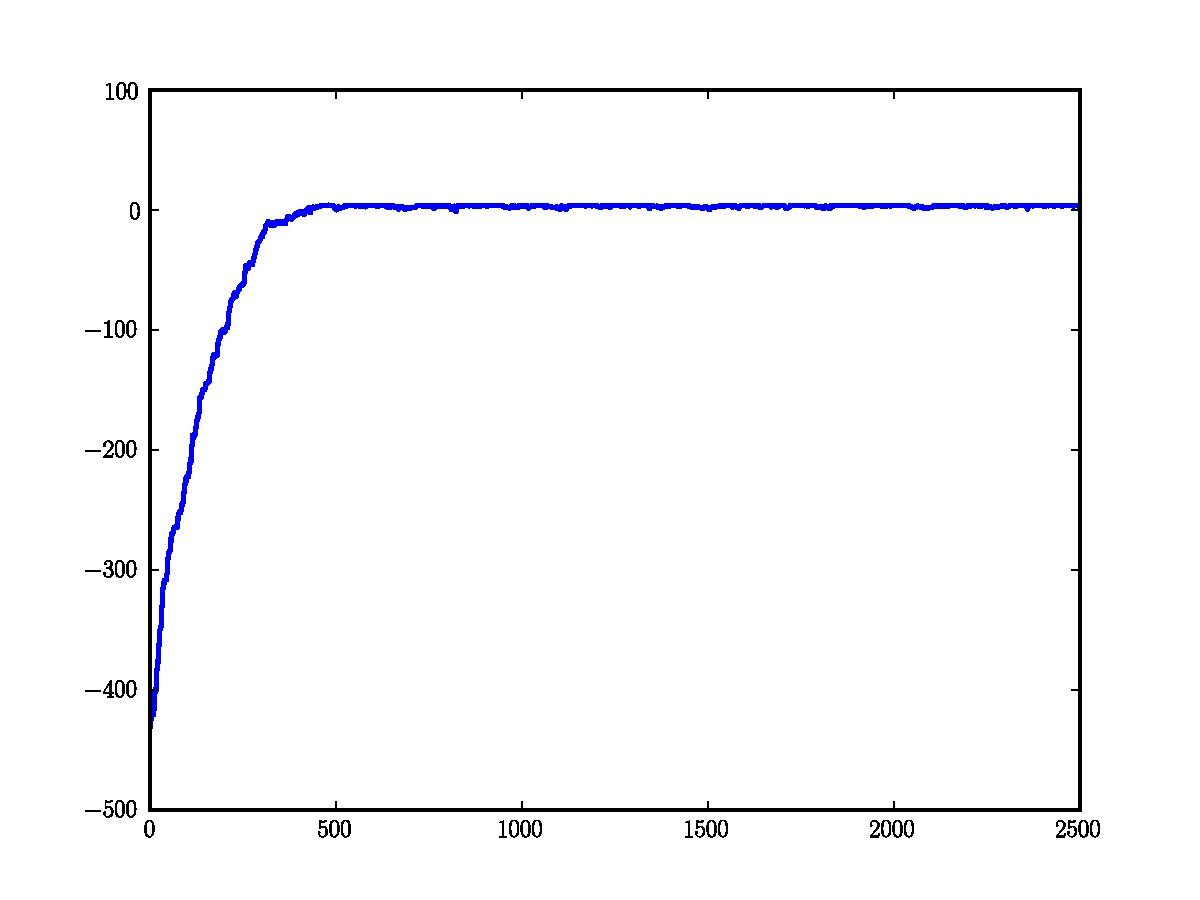
\includegraphics[width=\textwidth]{logprobs.pdf}
\caption{Log probabilities of our samples.}
\end{figure}

From this we can see that after between $300$ and $500$ iterations, we had converged to the correct distribution. We can visualize the path of our sampler by plotting the samples themselves:
\begin{figure}[h]
\centering
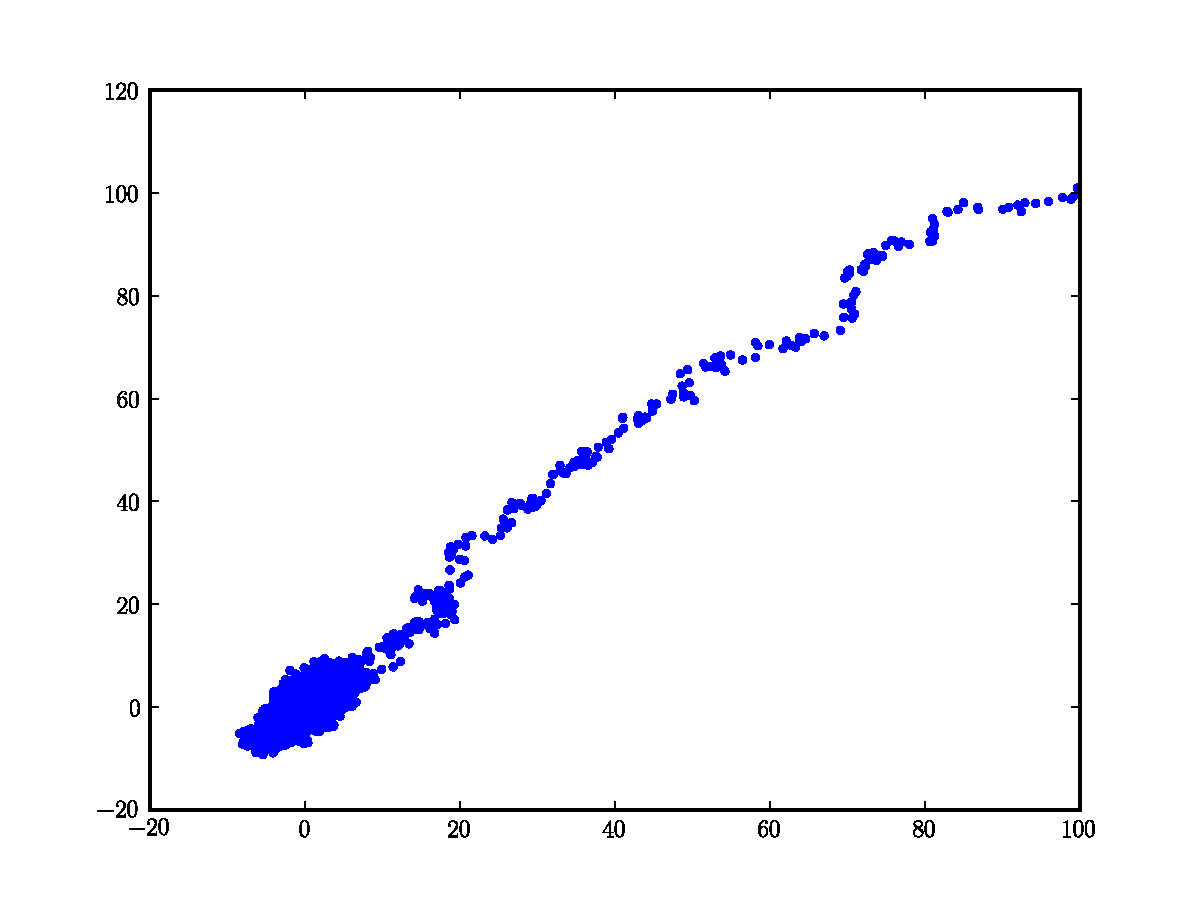
\includegraphics[width=\textwidth]{samples.pdf}
\caption{Samples from the Metropolis algorithm.}
\end{figure}

\begin{problem}
Using $\mu$ and $\Sigma$ as defined previously and using an initial state $\mathbf{x} = \left[ \begin{array}{cc} 1000 & -1000 \end{array} \right]$ run your Metropolis sampler for $10000$ iterations. Plot the log probs as well as the samples. How long did it take to converge?
\end{problem}